\documentclass[10pt,a4paper]{article}
\usepackage[margin=21mm,headheight=15pt]{geometry}
\usepackage[T1]{fontenc}
\usepackage{lmodern,amsmath,amssymb,tikz,graphicx,hyperref,fancyhdr,enumitem}
\usetikzlibrary{arrows.meta,positioning,calc,decorations.pathmorphing}
\definecolor{ink}{RGB}{20,53,78}
\hypersetup{colorlinks=true,urlcolor=ink,linkcolor=ink}
\setlength{\parindent}{0pt}\setlength{\parskip}{5pt}
\emergencystretch=3em
\pagestyle{fancy}\fancyhf{}\fancyfoot[C]{\thepage}
\renewcommand{\headrulewidth}{.3pt}
\newcommand{\task}[2]{\par\medskip{\color{ink}\Large\bfseries #1. #2}\par\smallskip}
\newcommand{\answer}{\par\smallskip\textbf{Worked reasoning.} }
\setlist[enumerate]{label=\textbf{(\alph*)},leftmargin=7mm,itemsep=7pt}
\begin{document}
\fancyhead[L]{\small Control of Dynamical Systems}
\fancyhead[R]{\small Laboratory 12}
{\color{ink}\LARGE\bfseries Laboratory 12}\par
{\large A synthetic process from identification to validation}\par
\textbf{Exercise sheet -- five integrated problems}\par
{\small\textbf{Evidence boundary.} Original hypothetical scenarios. Derive, calculate and justify decisions; every numerical record is synthetic. Figures are conceptual and not to scale.}
\smallskip\textbf{Shared nominal data.} Synthetic process: $G(s)=1.8e^{-0.6s}/(4s+1)$. Identification and validation use separate generated records. No parameter estimate or fitted response is a physical measurement.
\task{1}{Inferring an aggregate thermal process from a step}
The illustration shows a well-mixed thermal inventory followed by an ideal transport delay. The drawing supplies a physical interpretation, while the declared parameters define a synthetic teaching model.
\begin{center}\resizebox{\ifdim\width>.98\linewidth.98\linewidth\else\width\fi}{!}{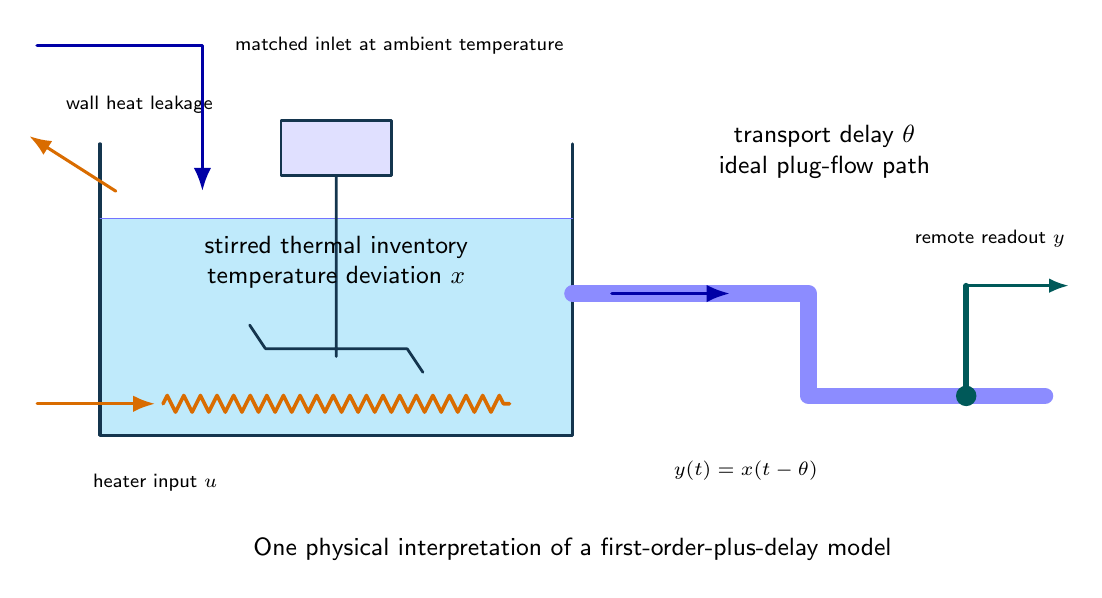
\begin{tikzpicture}[
font=\sffamily\small,>=Latex,line cap=round,line join=round,
wall/.style={draw=ink,line width=1.2pt,fill=blue!5},
water/.style={fill=cyan!25,draw=none},
metal/.style={draw=ink,fill=blue!12,line width=.9pt},
flow/.style={->,draw=blue!65!black,line width=1.2pt},
heat/.style={->,draw=orange!85!black,line width=1.1pt},
measure/.style={->,draw=teal!70!black,line width=.9pt},
dim/.style={<->,draw=ink!65,line width=.6pt},
spring/.style={draw=ink,decorate,decoration={coil,aspect=.5,segment length=4pt,amplitude=3pt}},
wire/.style={draw=ink,line width=1pt},
lab/.style={align=center,font=\sffamily\small},
smalllab/.style={align=center,font=\sffamily\scriptsize}]

\fill[water](1,.7)rectangle(7,3.45);
\draw[wall,fill=none](1,4.4)--(1,.7)--(7,.7)--(7,4.4);
\draw[blue!55](1,3.45)--(7,3.45);
\draw[metal](3.3,4)rectangle(4.7,4.7);
\draw[wire](4,4)--(4,1.7)(3.1,1.8)--(4.9,1.8)(3.1,1.8)--(2.9,2.1)(4.9,1.8)--(5.1,1.5);
\draw[orange!85!black,line width=1.3pt,decorate,decoration={zigzag,segment length=6pt,amplitude=3pt}](1.8,1.1)--(6.2,1.1);
\draw[heat](.2,1.1)--(1.7,1.1);
\node[smalllab]at(1.7,.1){heater input $u$};
\node[lab]at(4,2.9){stirred thermal inventory\\temperature deviation $x$};
\draw[heat](1.2,3.8)--(.1,4.5);
\node[smalllab]at(1.5,4.9){wall heat leakage};
\draw[flow](.2,5.65)--(2.3,5.65)--(2.3,3.8);
\node[smalllab]at(4.8,5.65){matched inlet at ambient temperature};
\draw[blue!45,line width=6pt](7,2.5)--(10,2.5)--(10,1.2)--(13,1.2);
\draw[flow](7.5,2.5)--(9,2.5);
\draw[teal!70!black,line width=2pt](12,1.2)--(12,2.6);
\fill[teal!70!black](12,1.2)circle(.13);
\draw[measure](12,2.6)--(13.3,2.6);
\node[smalllab]at(12.3,3.2){remote readout $y$};
\node[lab]at(10.2,4.3){transport delay $\theta$\\ideal plug-flow path};
\node[smalllab]at(9.2,.25){$y(t)=x(t-\theta)$};
\node[lab]at(7,-.75){One physical interpretation of a first-order-plus-delay model};
\end{tikzpicture}
}\par{\small A stirred thermal inventory followed by ideal transport is one possible physical interpretation of the identified transfer function. The effective conductance includes wall leakage and through-flow heat removal. Its fitted gain and time constant do not separately determine capacity, conductance and heater efficiency.}\end{center}
\begin{enumerate}
\item A synthetic process is $G(s)=K e^{-\theta s}/(\tau s+1)$ with $K=1.8$, $\tau=4$ s and $\theta=0.6$ s. A 2-unit step starts at $t_0=2$ s. Derive the zero-state output and find its final value and the time at which it reaches 63.212 percent of that final value.
\item In a deliberately noise-free synthetic step record with amplitude 2, the final output is 3.6, onset occurs 0.6 s after input changes, and the 63.212 percent point occurs 4 s after onset. Recover K, delay and time constant. Explain two obstacles with noisy sampled data.
\item For $C\dot x=\eta u-Hx$ followed by pure delay, relate $K,\tau$ to $C,\eta,H$. Show that $K=1.8$, $\tau=4$ do not uniquely identify all three physical parameters.
\end{enumerate}
\vfill{\small\textbf{Submission.} Show the model, intermediate reasoning, units and a conclusion addressing the stated requirements.}

\newpage
\task{2}{Fitting a delayed model without leaking validation information}
Fit only the training record, using an admissible parameterization. Keep independent excitation and noise for validation, and examine how the numerical delay representation affects optimization.
\begin{enumerate}
\item Write a least-squares objective for fitting K, time constant and delay to sampled step data. Propose a positive-parameter reparameterization and explain its limitation when zero delay is a plausible model.
\item Explain why reporting only training RMSE after fitting a noisy step response gives incomplete evidence. Specify a held-out synthetic input record and noise-generation procedure that avoids reusing the training noise.
\item What happens if a gradient-based fit represents delay only by a buffer rounded to an integer number of fixed time steps? Propose a more informative fitting representation and a subsequent implementation check.
\end{enumerate}
\vfill{\small\textbf{Submission.} Show the model, intermediate reasoning, units and a conclusion addressing the stated requirements.}

\newpage
\task{3}{A held-out multistep test with a statistical reference}
The validation record uses new input transitions and independent noise. Interpret residual magnitude using a specified stochastic model rather than claiming a perfect model from one small RMSE.
\begin{center}\resizebox{\ifdim\width>.98\linewidth.98\linewidth\else\width\fi}{!}{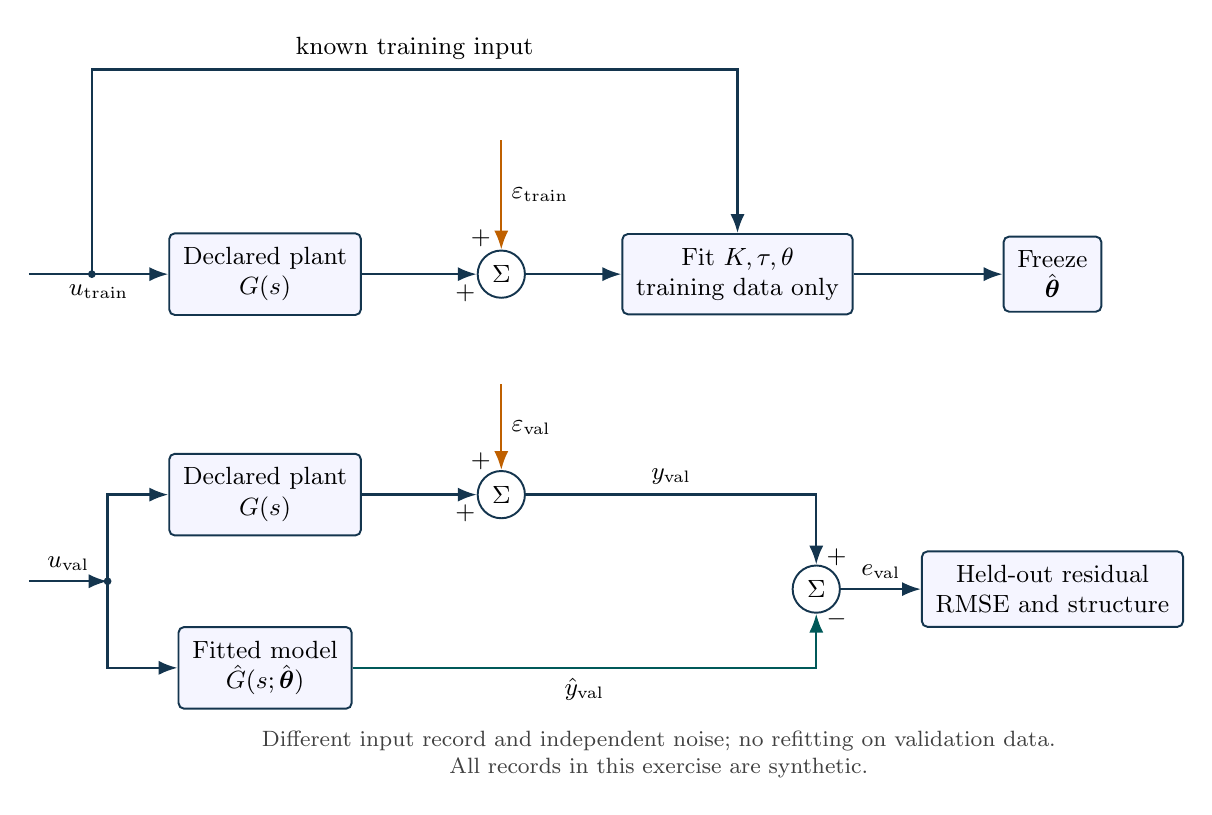
\begin{tikzpicture}[x=1cm,y=1cm,>=Latex,font=\small,
block/.style={draw=ink,fill=blue!4,rounded corners=2pt,minimum height=9mm,align=center,line width=.7pt,inner sep=5pt},
sum/.style={circle,draw=ink,fill=white,minimum size=6mm,inner sep=0pt,line width=.7pt},
sig/.style={->,draw=ink,line width=.85pt},
fb/.style={->,draw=teal!70!black,line width=.85pt},
dist/.style={->,draw=orange!75!black,line width=.85pt},
tap/.style={circle,fill=ink,inner sep=1.4pt},
note/.style={font=\footnotesize,align=center,text=black!75}]

\node[block](plant)at(3,1.5){Declared plant\\$G(s)$};
\node[sum](noise)at(6,1.5){$\Sigma$};
\node[block](fit)at(9,1.5){Fit $K,\tau,\theta$\\training data only};
\node[block](freeze)at(13,1.5){Freeze\\$\hat{\boldsymbol\theta}$};
\draw[sig](0,1.5)--node[below]{$u_{\mathrm{train}}$}(plant);
\draw[sig](plant)--node[pos=.9,below]{$+$}(noise);
\draw[dist](6,3.2)--node[right]{$\varepsilon_{\mathrm{train}}$}node[pos=.9,left]{$+$}(noise);
\draw[sig](noise)--(fit);\draw[sig](fit)--(freeze);
\draw[sig](.8,1.5)--(.8,4.1)--node[above]{known training input}(9,4.1)--(fit.north);
\fill[ink](.8,1.5)circle(1.4pt);
\node[block](truth)at(3,-1.3){Declared plant\\$G(s)$};
\node[block](pred)at(3,-3.5){Fitted model\\$\hat G(s;\hat{\boldsymbol\theta})$};
\node[sum](nv)at(6,-1.3){$\Sigma$};
\node[sum](err)at(10,-2.5){$\Sigma$};
\node[block](metric)at(13,-2.5){Held-out residual\\RMSE and structure};
\draw[sig](0,-2.4)--node[above]{$u_{\mathrm{val}}$}(1,-2.4);
\draw[sig](1,-2.4)--(1,-1.3)--(truth);
\draw[sig](1,-2.4)--(1,-3.5)--(pred);
\fill[ink](1,-2.4)circle(1.4pt);
\draw[sig](truth)--node[pos=.9,below]{$+$}(nv);
\draw[dist](6,.1)--node[right]{$\varepsilon_{\mathrm{val}}$}node[pos=.9,left]{$+$}(nv);
\draw[sig](nv)--node[above]{$y_{\mathrm{val}}$}(10,-1.3)--node[pos=.9,right]{$+$}(err);
\draw[fb](pred)--node[below]{$\hat y_{\mathrm{val}}$}(10,-3.5)--node[pos=.9,right]{$-$}(err);
\draw[sig](err)--node[above]{$e_{\mathrm{val}}$}(metric);
\node[note]at(8,-4.6){Different input record and independent noise; no refitting on validation data.\\All records in this exercise are synthetic.};

\end{tikzpicture}
}\par{\small Training selects parameters; held-out validation freezes them. Separate noise records avoid reusing training residuals as validation evidence.}\end{center}
\begin{enumerate}
\item Use input increments $+1$ at 1 s, $-0.6$ at 8 s, $+1.1$ at 15 s and $-0.8$ at 22 s. Write the exact synthetic model output and find its eventual equilibrium.
\item Validation adds independent zero-mean Gaussian noise of standard deviation 0.015. Explain the expected mean squared residual for a perfect deterministic model. Does a realized RMSE of 0.0145 prove the identified dynamics are exact?
\item For a perfect fixed deterministic model and $N=400$ independent Gaussian validation errors with $\sigma=0.015$, derive a central 95 percent reference interval for realized RMSE. Explain why it is not a confidence interval proving the fitted dynamics correct.
\end{enumerate}
\vfill{\small\textbf{Submission.} Show the model, intermediate reasoning, units and a conclusion addressing the stated requirements.}

\newpage
\task{4}{Tuning a PI law subject to uncertain steady capability}
Treat the tuning rule as a proposal and separately test whether the actuator can maintain the requested operating point under gain uncertainty and a constant disturbance.
\begin{enumerate}
\item Use $k_p=\tau/[K(\lambda+\theta)]$, $k_i=k_p/\tau$ with $\lambda=2$ s and nominal parameters. Calculate both gains and their changes if the assumed delay rises to 0.9 s.
\item The process input is constrained to $[0,2]$, and the reference is one. A constant disturbance of $-0.2$ is added inside the first-order state equation as $\tau\dot y=-y+Ku(t-\theta)-0.2$. Find the required equilibrium input before and after the disturbance.
\item Suppose the true gain lies in $[1.5,2.1]$, $u\in[0,2]$, and the disturbance in the state equation is $-0.2$. Find the largest reference guaranteed feasible at equilibrium for all allowed gains. Can increasing $\lambda$ make a reference of 3 feasible?
\end{enumerate}
\vfill{\small\textbf{Submission.} Show the model, intermediate reasoning, units and a conclusion addressing the stated requirements.}

\newpage
\task{5}{Implementing a noninteger transport delay}
The nominal simulation uses an exactly aligned delay, while a fitted delay need not align with the numerical grid. Preserve this distinction in uncertainty tests and reproduction notes.
\begin{enumerate}
\item Let $h=0.01$ s and delay 0.6 s, with zero-based indexing. Derive the exact held-input plant update and state which stored control sample is used at index k. Specify the first index at which an initial command $u_0$ influences the update.
\item The fitted parameters are approximately $[1.800025,3.993491,0.604289]$. Describe how to evaluate delay and gain uncertainty without claiming physical validation. Include training/validation separation, actuator limits and a numerical convergence check.
\item For $\theta=qh+\delta$ with integer $q$ and $0\le\delta<h$, derive the exact held-input update of the first-order process over one step. Identify both historical input samples used and apply the indexing rule to $\theta=0.604289$ s, $h=0.01$ s.
\end{enumerate}
\vfill{\small\textbf{Submission.} Show the model, intermediate reasoning, units and a conclusion addressing the stated requirements.}

\end{document}
